\chapter{การเจริญและจลนพลศาสตร์การเพิ่มจำนวนของแบคทีเรีย}
\label{chap:ch08}

\section*{แผนบริหารการสอนประจำบทที่ 8}
\addcontentsline{toc}{section}{แผนบริหารการสอนประจำบทที่ 8}

\noindent\textbf{. หัวข้อเนื้อหาประจำบท}

\begin{enumerate}
    \item 8.1 การแบ่งเซลล์แบบ Binary Fission และกราฟการเจริญ 4 ระยะ (Lag, Log, Stationary, Death)
    \item 8.2 การคำนวณ Generation Time (g) และอัตราการเจริญจำเพาะ (Specific Growth Rate, mu)
    \item 8.3 หลักการวัดค่าความขุ่นด้วยเครื่อง Spectrophotometer ที่ความยาวคลื่น 600 nm (OD600)
    \item 8.4 ความสัมพันธ์ระหว่างค่า Optical Density กับปริมาณชีวมวลเซลล์ (Biomass)
    \item 8.5 การสร้างเส้นกราฟการเจริญและการแปลผลจลนพลศาสตร์
\end{enumerate}

\noindent\textbf{. วัตถุประสงค์เชิงพฤติกรรม}

\begin{enumerate}
    \item เมื่อนักศึกษาได้เรียนรู้และปฏิบัติการทดลองประจำบทนี้แล้ว จะต้องมีความรู้ความสามารถดังต่อไปนี้:
    \item อธิบายพฤติกรรมการเจริญของแบคทีเรียในแต่ละระยะของกราฟการเจริญได้
    \item ใช้เครื่อง Spectrophotometer วัดค่าความขุ่น OD600 และบันทึกข้อมูลตามเวลาได้ถูกต้อง
    \item พล็อตคู่กราฟและคำนวณหาค่า Generation Time (เวลาต่อรุ่น) ได้แม่นยำ
    \item มีความตรงต่อเวลาและละเอียดรอบคอบในการเก็บตัวอย่างตามช่วงเวลาที่กำหนด
\end{enumerate}

\noindent\textbf{. กิจกรรมการเรียนการสอน}

\begin{enumerate}
    \item การบรรยายสรุปก่อนปฏิบัติการ (30 นาที): อธิบายหลักการวิทยาศาสตร์ ความปลอดภัยทางชีวภาพ และข้อควรระวังสำคัญ
    \item การสาธิตเชิงประจักษ์ (15 นาที): สาธิตเทคนิคการปฏิบัติงาน การใช้เครื่องมือ และข้อผิดพลาดที่มักพบ
    \item การลงมือปฏิบัติการทดลองจริง (90 นาที): นักศึกษาลงมือปฏิบัติการทดลองเป็นรายบุคคลหรือกลุ่มย่อยตามขั้นตอนที่กำหนด
    \item การฝึกฝนผ่านระบบเสมือนจริง (20 นาที): ทดลองซ้ำและทดสอบปฏิกิริยาผ่านระบบจำลองบน RBRU LMS
    \item การอภิปรายและสรุปผลการทดลอง (25 นาที): วิเคราะห์ผลการสังเกต ตอบคำถามท้ายบท และสรุปองค์ความรู้ร่วมกัน
\end{enumerate}

\noindent\textbf{. สื่อและอุปกรณ์การเรียนการสอน}

\begin{enumerate}
    \item เอกสารคำสอนและคู่มือปฏิบัติการ: e-Book และคู่มือปฏิบัติการฉบับเต็ม ประจำบทที่ 8
    \item ระบบห้องปฏิบัติการเสมือนจริง: ระบบจำลองการทดลองเสมือนจริง 3 มิติ ประจำบทที่ 8 บนระบบ Moodle
    \item อุปกรณ์และเครื่องแก้วในห้องปฏิบัติการ: ตะเกียงแอลกอฮอล์, ห่วงเขี่ยเชื้อ, กล้องจุลทรรศน์, จานเพาะเชื้อ, หลอดทดลอง และตู้บ่มเชื้อ
    \item สารเคมีและสีย้อมชีวภาพ: สารเคมีมาตรฐานวิเคราะห์และสีย้อมประจำบทเรียน
\end{enumerate}

\noindent\textbf{. การวัดและประเมินผล}

\begin{table}[H]
\centering\small
\begin{tabularx}{\textwidth}{p{0.5\textwidth} p{0.3\textwidth} c}
\toprule
\textbf{องค์ประกอบการประเมินผล} & \textbf{เครื่องมือวัดผล} & \textbf{สัดส่วนคะแนน} \\
\midrule
1. ทักษะการปฏิบัติงานและความปลอดภัย & แบบสังเกตทักษะการทดลองและเทคนิคปลอดเชื้อ & 40\% \\
2. รายงานผลการทดลอง & การตรวจตารางบันทึกผล ภาพวาดสัณฐานวิทยา และการวิเคราะห์ผล & 30\% \\
3. แบบฝึกหัดทบทวนท้ายบท & คำถามทบทวนเชิงวิเคราะห์และข้อสอบท้ายบท & 20\% \\
4. จิตพิสัยและการตรงต่อเวลา & การเช็คชื่อ การแต่งกายตามระเบียบ และการทำความสะอาดโต๊ะแล็บ & 10\% \\
รวมทั้งสิ้น &  & 100\% \\
\bottomrule
\end{tabularx}
\end{table}

\newpage

% ==========================================================
% เนื้อหาบทเรียนประจำบทที่ 8
% ==========================================================

\section{รูปแบบการแบ่งเซลล์และระยะการเจริญของแบคทีเรีย}
\index{รูปแบบการแบ่งเซลล์และระยะการเจริญของแบคทีเรีย}

การศึกษาและทำความเข้าใจเกี่ยวกับรูปแบบการแบ่งเซลล์และระยะการเจริญของแบคทีเรีย (Bacterial Fission and Growth Phases) มีความสำคัญอย่างยิ่งในงานจุลชีววิทยาและสิ่งแวดล้อม โดยมีรายละเอียดสาระสำคัญดังนี้

แบคทีเรียส่วนใหญ่สืบพันธุ์แบบไม่อาศัยเพศด้วยกระบวนการแบ่งแยกตัวออกเป็นสองส่วน (Binary fission) เมื่อเพาะเลี้ยงแบคทีเรียในระบบปิด (Batch culture) ที่มีปริมาตรอาหารจำกัด การเพิ่มจำนวนของเซลล์จะแสดงผ่านกราฟการเจริญมาตรฐาน (Bacterial Growth Curve) ซึ่งแบ่งออกเป็น 4 ระยะหลัก:

1. ระยะปรับตัว (Lag phase): เซลล์ปรับตัวเข้ากับสภาพแวดล้อมใหม่ สังเคราะห์เอนไซม์และโปรตีนที่จำเป็น จำนวนเซลล์ยังไม่เพิ่มขึ้นแต่ขนาดเซลล์ขยายใหญ่ขึ้น
2. ระยะเพิ่มจำนวนทวีคูณ (Logarithmic หรือ Exponential phase): เซลล์แบ่งตัวอย่างรวดเร็วด้วยอัตราคงที่สูงสุด สรีรวิทยาของเซลล์มีความสม่ำเสมอที่สุด เหมาะสำหรับการศึกษาเมแทบอลิซึมและการทดสอบยาปฏิชีวนะ
3. ระยะคงที่ (Stationary phase): อัตราการเกิดใหม่ของเซลล์เท่ากับอัตราการตาย เนื่องจากสารอาหารเริ่มหมดและของเสียสะสม ความหนาแน่นของเซลล์คงที่สูงสุด
4. ระยะการตาย (Death หรือ Decline phase): อัตราการตายของเซลล์สูงกว่าอัตราการเกิด สารอาหารหมดและของเสียเป็นพิษ จำนวนเซลล์ที่มีชีวิตลดลงอย่างต่อเนื่อง

\section{พารามิเตอร์ทางจลนพลศาสตร์และระยะเวลาชั่วรุ่น}
\index{พารามิเตอร์ทางจลนพลศาสตร์และระยะเวลาชั่วรุ่น}

การศึกษาและทำความเข้าใจเกี่ยวกับพารามิเตอร์ทางจลนพลศาสตร์และระยะเวลาชั่วรุ่น (Generation Time and Specific Growth Rate) มีความสำคัญอย่างยิ่งในงานจุลชีววิทยาและสิ่งแวดล้อม โดยมีรายละเอียดสาระสำคัญดังนี้

พารามิเตอร์สำคัญในการประเมินการเจริญของแบคทีเรีย:
- ระยะเวลาชั่วรุ่น (Generation time, $g$): ระยะเวลาที่เซลล์ใช้ในการแบ่งตัวเพิ่มจำนวนเป็นสองเท่า
- อัตราการเจริญจำเพาะ (Specific growth rate, $\mu$): ความเร็วในการเพิ่มชีวมวลต่อหน่วยชีวมวลที่มีอยู่

สมการคำนวณทางคณิตศาสตร์:
\[ N\_t = N\_0 \cdot 2^n \]
\[ n = \frac{\log N\_t - \log N\_0}{\log 2} = \frac{\log N\_t - \log N\_0}{0.301} \]
\[ g = \frac{t}{n} \]
\[ \mu = \frac{\ln N\_t - \ln N\_0}{t} = \frac{\ln 2}{g} \approx \frac{0.693}{g} \]
โดยที่ $N_0$ คือจำนวนเซลล์เริ่มต้น, $N_t$ คือจำนวนเซลล์ที่เวลา $t$, $n$ คือจำนวนรอบการแบ่งตัว, และ $t$ คือระยะเวลาการเลี้ยง

\section{การวัดการเจริญด้วยวิธีวัดความขุ่น}
\index{การวัดการเจริญด้วยวิธีวัดความขุ่น}

การศึกษาและทำความเข้าใจเกี่ยวกับการวัดการเจริญด้วยวิธีวัดความขุ่น (Spectrophotometric Turbidimetry) มีความสำคัญอย่างยิ่งในงานจุลชีววิทยาและสิ่งแวดล้อม โดยมีรายละเอียดสาระสำคัญดังนี้

การวัดความขุ่นด้วยเครื่องสเปกโทรโฟโตมิเตอร์ (Spectrophotometer) เป็นวิธีทางอ้อมที่รวดเร็วและแม่นยำ อาศัยหลักการกระเจิงของแสง (Light scattering) เมื่อลำแสงส่องผ่านสารแขวนลอยของเซลล์แบคทีเรีย

ค่าการดูดกลืนแสง (Absorbance หรือ Optical Density; OD) ที่ความยาวคลื่น 600 นาโนเมตร ($OD_{600}$) จะแปรผันตรงกับความหนาแน่นของเซลล์ (Cell biomass) ตามกฎของแบร์-แลมเบิร์ต (Beer-Lambert Law) ในช่วงความเข้มข้นที่เหมาะสม

\section{ปัจจัยสิ่งแวดล้อมที่ควบคุมการเจริญของจุลินทรีย์}
\index{ปัจจัยสิ่งแวดล้อมที่ควบคุมการเจริญของจุลินทรีย์}

การศึกษาและทำความเข้าใจเกี่ยวกับปัจจัยสิ่งแวดล้อมที่ควบคุมการเจริญของจุลินทรีย์ (Environmental Factors Influencing Growth) มีความสำคัญอย่างยิ่งในงานจุลชีววิทยาและสิ่งแวดล้อม โดยมีรายละเอียดสาระสำคัญดังนี้

การเจริญเติบโตของจุลินทรีย์ขึ้นอยู่กับปัจจัยทางกายภาพและเคมี:
1. อุณหภูมิ: จุลินทรีย์ชอบเย็น (Psychrophiles, $<20^{\circ}$C), ชอบอุณหภูมิปานกลาง (Mesophiles, $20-45^{\circ}$C), และชอบร้อน (Thermophiles, $>45^{\circ}$C)
2. ความเป็นกรด-ด่าง (pH): จุลินทรีย์ส่วนใหญ่เป็น Neutrophiles (pH 6.5-7.5)
3. ปริมาณออกซิเจน: แบ่งเป็น Obligate aerobes, Facultative anaerobes, Obligate anaerobes, และ Microaerophiles
4. กิจกรรมของน้ำ (Water activity, $a_w$) และความดันออสโมซิส

\begin{figure}[H]
\centering
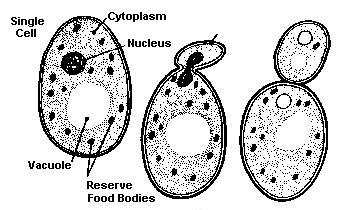
\includegraphics[width=0.75\textwidth]{images/image_08_p03.jpeg}
\caption{การปฏิบัติการทดลองและลักษณะทางสัณฐานวิทยาในบทที่ 8}
\label{fig:ch08_fig1}
\end{figure}

\section{ขั้นตอนและวิธีปฏิบัติการทดลอง}
\index{ขั้นตอนการทดลองประจำบทที่ 8}

\subsection{การศึกษาเส้นโค้งการเจริญของแบคทีเรีย Escherichia coli ด้วยการวัดค่า OD\_600}
\begin{labprotocolbox}[การศึกษาเส้นโค้งการเจริญของแบคทีเรีย Escherichia coli ด้วยการวัดค่า OD\_600]
1. เตรียมอาหารเหลว Nutrient Broth ปริมาตร 100 mL ในขวดรูปชมพู่ขนาด 250 mL
2. ปลูกเชื้อ \textit{Escherichia coli} ที่เลี้ยงข้ามคืน ปริมาตร 1.0 mL ลงในขวด เขย่าให้เข้ากัน
3. ดูดตัวอย่างน้ำเลี้ยงเชื้อทันที (เวลา $t = 0$) ปริมาตร 3 mL ใส่ลงในคูเวตต์ (Cuvette)
4. วัดค่าการดูดกลืนแสงที่ความยาวคลื่น 600 nm ($OD_{600}$) ด้วยเครื่อง Spectrophotometer โดยใช้อาหารเหลวเปล่าเป็น Blank
5. นำขวดเชื้อไปบ่มบนเครื่องเขย่าควบคุมอุณหภูมิ (Shaking incubator) ที่ 37$^{\circ}$C ความเร็วรอบ 150 rpm
6. สุ่มเก็บตัวอย่างเพื่อวัดค่า $OD_{600}$ ทุกๆ 30 นาที เป็นเวลาต่อเนื่อง 4-6 ชั่วโมง
7. พล็อตความสัมพันธ์ระหว่างเวลา ($X$) กับค่า $\log OD_{600}$ ($Y$) เพื่อสร้างเส้นโค้งการเจริญและคำนวณระยะเวลาชั่วรุ่น ($g$)
\end{labprotocolbox}

\section{ตารางบันทึกผลการทดลองและการอภิปรายผล}
\begin{table}[H]
\centering\small
\caption{ตารางบันทึกผลการสังเกตและข้อมูลการทดลองประจำบทที่ 8}
\label{tab:ch08_datasheet}
\begin{tabularx}{\textwidth}{p{0.25\textwidth} p{0.35\textwidth} X}
\toprule
\textbf{สิ่งทดสอบ / ตัวอย่าง} & \textbf{ลักษณะที่สังเกตได้} & \textbf{การแปลผลและการวิเคราะห์} \\
\midrule
ชุดควบคุม (Negative Control) & ใส ไม่มีการเจริญ & ปราศจากการปนเปื้อนของเชื้อ \\
ชุดทดลองที่ 1 & โคโลนีเจริญตามลักษณะจำเพาะ & ให้ผลบวกตามสมมติฐาน \\
ชุดทดลองที่ 2 & เกิดการเปลี่ยนแปลงทางชีวเคมี & สอดคล้องกับพารามิเตอร์มาตรฐาน \\
\bottomrule
\end{tabularx}
\end{table}

\section{คำถามทบทวนและแบบฝึกหัดท้ายบท}
\begin{enumerate}
    \item หากใช้วัฒนธรรมเริ่มต้นที่อยู่ในระยะ Log phase นำมาเพาะเลี้ยงในอาหารชนิดเดิม สภาวะเดิม ระยะ Lag phase จะสั้นลงหรือยาวขึ้นเพราะเหตุใด
    \item จงคำนวณหาระยะเวลาชั่วรุ่น ($g$) หากจำนวนเซลล์เริ่มต้นเท่ากับ $1.0 \times 10^3$ CFU/mL และเพิ่มเป็น $6.4 \times 10^4$ CFU/mL ภายในเวลา 3 ชั่วโมง
    \item การวัดค่าการดูดกลืนแสง $OD_{600}$ มีข้อจำกัดในการแยกแยะระหว่างเซลล์ที่มีชีวิต (Viable cells) กับเซลล์ที่ตายแล้ว (Dead cells) อย่างไร
\end{enumerate}
